

\documentclass[twoside]{article}
\setlength{\oddsidemargin}{0.25 in}
\setlength{\evensidemargin}{-0.25 in}
\setlength{\topmargin}{-0.6 in}
\setlength{\textwidth}{6.5 in}
\setlength{\textheight}{8.5 in}
\setlength{\headsep}{0.75 in}
\setlength{\parindent}{0 in}
\setlength{\parskip}{0.1 in}

%
% ADD PACKAGES here:
%

\usepackage{amsmath,amsfonts,graphicx}

%
\newcounter{lecnum}
\renewcommand{\thepage}{\thelecnum-\arabic{page}}
\renewcommand{\thesection}{\thelecnum.\arabic{section}}
\renewcommand{\theequation}{\thelecnum.\arabic{equation}}
\renewcommand{\thefigure}{\thelecnum.\arabic{figure}}
\renewcommand{\thetable}{\thelecnum.\arabic{table}}

%
% The following macro is used to generate the header.
%
\newcommand{\lecture}[4]{
   \pagestyle{myheadings}
   \thispagestyle{plain}
   \newpage
   \setcounter{lecnum}{#1}
   \setcounter{page}{1}
   \noindent
   \begin{center}
   \framebox{
      \vbox{\vspace{2mm}
    \hbox to 6.28in { {\bf EE402 - Discrete Time Systems
	\hfill Spring 2018} }
       \vspace{4mm}
       \hbox to 6.28in { {\Large \hfill Lecture #1 \hfill} }
       \vspace{2mm}
       \hbox to 6.28in { {\it Lecturer: #2 \hfill } }
      \vspace{2mm}}
   }
   \end{center}
   \markboth{Lecture #1}{Lecture #1}

   \vspace*{4mm}
}


\renewcommand{\cite}[1]{[#1]}
\def\beginrefs{\begin{list}%
        {[\arabic{equation}]}{\usecounter{equation}
         \setlength{\leftmargin}{2.0truecm}\setlength{\labelsep}{0.4truecm}%
         \setlength{\labelwidth}{1.6truecm}}}
\def\endrefs{\end{list}}
\def\bibentry#1{\item[\hbox{[#1]}]}

%Use this command for a figure; it puts a figure in wherever you want it.
%usage: \fig{NUMBER}{SPACE-IN-INCHES}{CAPTION}
\newcommand{\fig}[3]{
			\vspace{#2}
			\begin{center}
			Figure \thelecnum.#1:~#3
			\end{center}
	}
% Use these for theorems, lemmas, proofs, etc.
\newtheorem{theorem}{Theorem}[lecnum]
\newtheorem{lemma}[theorem]{Lemma}
\newtheorem{proposition}[theorem]{Proposition}
\newtheorem{claim}[theorem]{Claim}
\newtheorem{corollary}[theorem]{Corollary}
\newtheorem{definition}[theorem]{Definition}
\newenvironment{proof}{{\bf Proof:}}{\hfill\rule{2mm}{2mm}}

% **** IF YOU WANT TO DEFINE ADDITIONAL MACROS FOR YOURSELF, PUT THEM HERE:

\begin{document}

% Lecture Details
\lecture{12}{Asst. Prof. M. Mert Ankarali}

\par

\section*{State-Space Representation of DT Systems}

State-space representation of a (causal \& finite dimensional) LTI CT system is given by
%
\begin{align*}
  \mathrm{Let} \ x(t) &\in \mathbb{R}^n \ , \ y(t) \in \mathbb{R}^m \ ,\  u(t) \in
  \mathbb{R}^r , \\
  \dot{x}(t) &= A x(t) + B u(t) , \\
  y(t) &= C x(t) + D u(t) , \\
  \mathrm{where} \ A &\in \mathbb{R}^{n \times n} \ , \ 
    B \in \mathbb{R}^{n \times r} \ ,\  C \in \mathbb{R}^{m \times n} \ , \ D \in \mathbb{R}^{m \times r}
\end{align*}
%
State-space representation of a (causal \& finite dimensional) LTI DT system is given by
%
\begin{align*}
  \mathrm{Let} \ x[k] &\in \mathbb{R}^n \ , \ y[k] \in \mathbb{R}^m \ ,\  u[k] \in
  \mathbb{R}^r , \\
  x[k+1] &= G x[k] + H u[k] , \\
  y[k] &= C x[k] + D u[k] , \\
  \mathrm{where} \ G &\in \mathbb{R}^{n \times n} \ , \ 
    H \in \mathbb{R}^{n \times r} \ ,\  C \in \mathbb{R}^{m \times n} \ , \ D \in \mathbb{R}^{m \times r}
\end{align*}
%
Depending on the values of $m$ and $r$ we have 
%
\begin{itemize}
  \item $m = r = 1$, the system represents a SISO system 
  \item $m > 1 \ , \  r < 1$, the system represents a MIMO system 
  \item $m = 1 \ , \ r > 1$, the system represents a MISO system 
  \item $m > 1  \ , \ r = 1$, the system represents a SIMO system 
\end{itemize}
%
for both CT and DT cases.

\textbf{State property of CT state-space models:} Given the initial time,
$t_0$ and state $x(t_0)$ and input $u(t)$ for $t_0 \leq t < t_f$ (with
$t_0 \ \& \ t_f$ arbitrary), we can compute the output $y(t)$ for 
$t_0 \leq t \leq t_f$ and the state $x(t)$ for $t_0 \leq t \leq t_f$. 

\textbf{State property of DT state-space models:} 
Given the state vector $x[k]$ and input $u[k]$ at an arbitrary time $k$, 
we can compute the the present output, $y[k]$, and next state $x[k+1]$.

Note that both definitions are not limited to LTI state-space models. 
Nonlinear and time-varying state-space models also are based on this 
definition. 

When a state-space representation includes minimum number of state 
variables, the representation is called minimal. 

\subsection*{Canonical State-Space Realizations of (SISO) DT Systems}

\subsubsection*{Reachable/Controllable Canonical Form}

For the sake of clarity let's assume that the system that we would
like to represent is a third order DT system with the following difference equation
and transfer function

\begin{align*}
y[k] &=  -a_1 y[k-1] - a_2 y[k-2] - a_3 y[k-3] 
+ b_0 x[k] + b_1 x[k-1] + b_2 x[k-2] + b_3 x[k-3] \\ 
Y(z) &= \frac{b_0 + b_1 z^{-1} + b_2 z^{-2} + b_3 z^{-3}}{1+ a_1 z^{-1} + a_2 z^{-2} + a_3 z^{-3}} X(z)
\end{align*}

We know that following block 
ram realizes this system structure
with minimum number of delay elements and it is a canonical
realization. Delay operation is directly
related with state and state evolution concept.
%
     \begin{center}
 \begin{minipage}[h]{0.7\linewidth}
     \begin{center}
       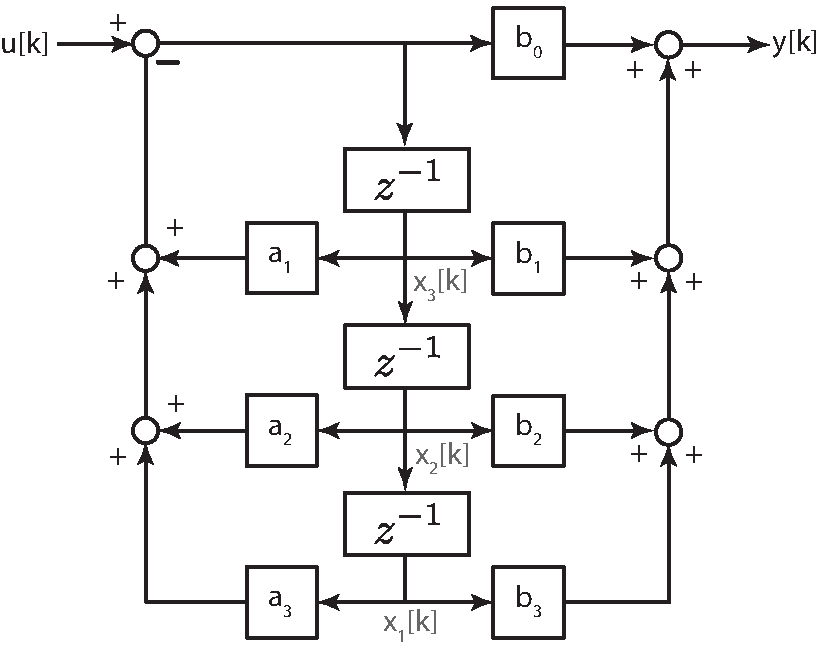
\includegraphics[width=\textwidth]{reachable}
     \end{center}
 \end{minipage}
     \end{center}
%
If we label the signals as given in the Figure,
state evolution equations can be derived as
%
\begin{align*}
X_1(z) = X_2(z) z^{-1}  \quad &\rightarrow \quad x_1[k+1] = x_2[k]
\\
X_2(z) = X_3(z) z^{-1}  \quad &\rightarrow \quad x_2[k+1] = x_3[k]
\\
X_3(z) = \left( U(z)  - \left( X_1(z) a_3 + X_2(z) a_2 + X_3(z) a_1 \right) \right) z^{-1}
\quad &\rightarrow \quad 
x_3[k+1] =  u[k] + x_1[k] (-a_3) + x_2[k] (-a_2) + x_3[k] (-a_1)
\end{align*}
%
where as output equation can be derived as
%
\begin{align*}
y[k] &= b_1 x_3[k] + b_2 x_2[k] + b_3 x_1[k]
b_0 u[k] - b_0 \left( a_1 x_3[k] + a_2 x_2[k] + a_3 x_1[k] \right)
\\
&= b_0 u[k] + (b_3 - b_0 a_3) x_1[k] + (b_2 - b_0 a_2) x_2[k] 
+ (b_1 - b_0 a_1) x_3[k] 
\end{align*}
%
If we gather these equations, we can obtain the state space form
%
\begin{align*}
  \mathbf{x}[k+1] &= \left[ \begin{array}{ccc} 0 & 1 & 0 \\ 0 & 0 & 1
    \\ -a_3 & -a_2 & -a_1 \end{array} \right] \mathbf{x}[k]
   + 
  \left[ \begin{array}{c} 0\\ 0 
    \\ 1 \end{array} \right] u[k]
\\
y[k] &= \left[ \begin{array}{ccc} (b_3 - b_0 a_3) &  (b_2 - b_0 a_2) &
                                                                       (b_1 - b_0 a_1) \end{array} \right]
+ b_0 u[k]
\end{align*}
%
where 
%
\begin{align*}
\mathbf{x} = \left[ \begin{array}{c} x_1[k] \\ x_2[k] \\
x_1[k] \end{array} \right] \quad , \quad
A = \left[ \begin{array}{ccc} 0 & 1 & 0 \\ 0 & 0 & 1
    \\ -a_3 & -a_2 & -a_1 \end{array} \right]
\quad , \quad 
B = \left[ \begin{array}{c} 0\\ 0 
    \\ 1 \end{array} \right]
\\ C = \left[ \begin{array}{ccc} (b_3 - b_0 a_3) &  (b_2 - b_0 a_2) &
   (b_1 - b_0 a_1) \end{array} \right]
\quad , \quad
D = b_0
\end{align*}
%
The form obtained with this approach is called
reachable/controllable canonical form. 

For a general $n^{th}$ order system reachable/controllable
canonical form has the following $A \ ,  B \ ,  C \ , \& \ D$
matrices
%
\begin{align*}
A &= \left[ \begin{array}{ccccc} 0 & 1 & 0 & \cdots & 0 \\ 0 & 0 & 1 &
                                                                      \cdots & 0
\\ \vdots & \vdots & \vdots & & \vdots
\\ 0 & 0 & 0 & \cdots & 1
    \\ -a_n & -a_{n-1} & -a_{n-2} & \cdots & -a_1 \end{array} \right]
\quad , \quad 
B = \left[ \begin{array}{c} 0\\ 0 \\ \vdots \\ 0
    \\ 1 \end{array} \right]
\\ C &= \left[ \begin{array}{ccccc} (b_n - b_0 a_n) 
  &  (b_{n-1} - b_0 a_{n-1}) & \cdots &  (b_2 - b_0 a_2) &
   (b_1 - b_0 a_1) \end{array} \right]
\quad , \quad
D = b_0
\end{align*}

\subsubsection*{Observable Canonical Form}

We also learnt a different type of canonical 
minimal realization which is illustrated 
in the Figure below
%
     \begin{center}
 \begin{minipage}[h]{0.6\linewidth}
     \begin{center}
       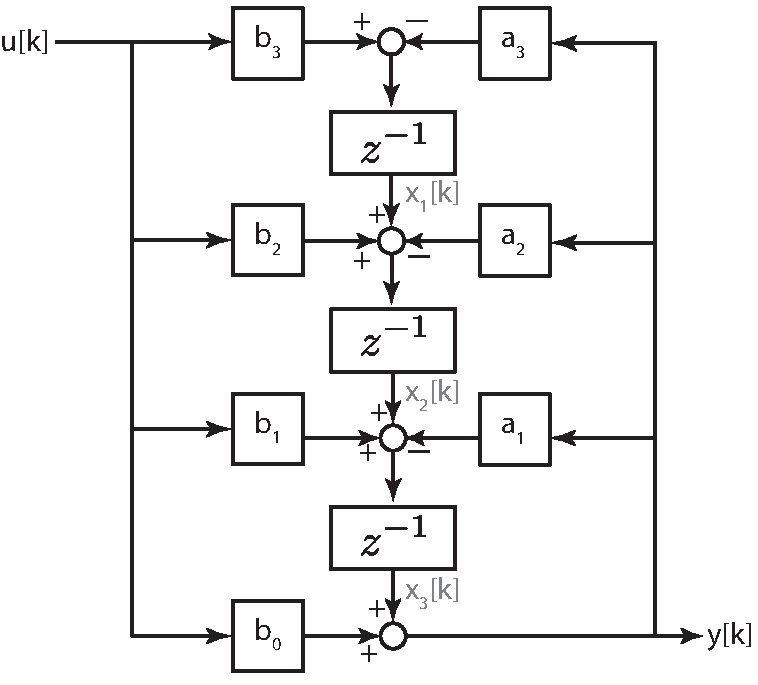
\includegraphics[width=\textwidth]{observable}
     \end{center}
 \end{minipage}
     \end{center}
%
If we label the signals as given in the Figure,
state evolution equations can be derived as
%
\begin{align*}
X_1(z) = \left( b_3 U(z) - a_3 \left( U(z) b_0 + X_3(z) \right) \right) z^{-1}
\quad &\rightarrow \quad x_1[k+1] = b_3 u[k] - a_3 \left( u[k] b_0 +
        x_3[k] \right)
\\
X_2(z) = \left( b_2 U(z) + X_1(z) - a_2 \left( U(z) b_0 + X_3(z) \right) \right) z^{-1}
\quad &\rightarrow \quad x_2[k+1] = b_2 u[k] + x_1[k] - a_2 \left( u[k] b_0 +
        x_3[k] \right)
\\
X_3(z) = \left( b_1 U(z) + X_2(z) - a_1 \left( U(z) b_0 + X_3(z) \right) \right) z^{-1}
\quad &\rightarrow \quad x_3[k+1] = b_1 u[k] + x_2[k] - a_1 \left( u[k] b_0 +
        x_3[k] \right)
\end{align*}
%
where as output equation can be derived as
%
\begin{align*}
y[k] &= b_0 u[k] + x_3[k]
\end{align*}
%
If we combine the state and output equations, we
can obtain the state space form as
%
%
\begin{align*}
  \mathbf{x}[k+1] &= \left[ \begin{array}{ccc} 0 & 0 & -a_3 \\ 1 & 0 & -a_2
    \\ 0 & 1 & -a_1 \end{array} \right] \mathbf{x}[k]
   + 
  \left[ \begin{array}{c} b_3 - b_0 a_3 \\ b_2 - b_0 a_2
    \\ b_1 - b_0 a_1 \end{array} \right] u[k]
\\
y[k] &= \left[ \begin{array}{ccc} 0 & 0 & 1 \end{array} \right]
+ b_0 u[k]
\end{align*}
%
where 
%
\begin{align*}
\mathbf{x} = \left[ \begin{array}{c} x_1[k] \\ x_2[k] \\
x_1[k] \end{array} \right] \quad , \quad
A = \left[ \begin{array}{ccc} 0 & 0 & -a_3 \\ 1 & 0 & -a_2
    \\ 0 & 1 & -a_1 \end{array} \right]
\quad , \quad 
B = \left[ \begin{array}{c} b_3 - b_0 a_3 \\ b_2 - b_0 a_2
    \\ b_1 - b_0 a_1 \end{array} \right]
\quad , \quad
C = \left[ \begin{array}{ccc} 0 & 0 & 1 \end{array} \right]
\quad , \quad
D = b_0
\end{align*}
%

The form obtained with this approach is called
observable canonical form. 

For a general $n^{th}$ order system observable
canonical form has the following $A \ ,  B \ ,  C \ , \& \ D$
matrices
%
\begin{align*}
A &= \left[ \begin{array}{ccccc} 0 & 0 & \cdots & 0 & -a_{n} 
              \\ 1 & 0 & \cdots & 0 & -a_{n-1} 
\\ \vdots & \vdots & \vdots & \vdots & \vdots
\\ 0 & 0 & \cdots & 0 & -a_2
    \\ 0 & 0 & \cdots & 1 & -a_1 \end{array} \right]
\quad , \quad 
B = \left[ \begin{array}{c} (b_n - b_0 a_n)  \\ (b_{n-1} - b_0
             a_{n-1}) \\ \vdots \\ (b_2 - b_0 a_2) \\   (b_1 - b_0
             a_1) 
\end{array} \right]
\\ C &= \left[ \begin{array}{ccccc} 0 & 0 & \cdots &  0 & 1 \end{array} \right]
\quad , \quad
D = b_0
\end{align*}
%
\subsubsection*{Diagonal Canonical Form}

If the pulse transfer function of the system 
has distinct poles, we can expand it 
using partial fraction expansion 
%
\begin{align*}
Y(z) &= \frac{b_0 + b_1 z^{-1} + b_2 z^{-2} + b_3 z^{-3}}{1+ a_1
       z^{-1} + a_2 z^{-2} + a_3 z^{-3}} X(z)
\\
&= \left( b_0 + \frac{c_1}{z - p_1} + \frac{c_2}{z - p_2}
+ \frac{c_3}{z - p_3} \right) X(z)
\end{align*}
%
It is possible to realize this expanded form in block diagram 
form as given in the Figure below.
%
     \begin{center}
 \begin{minipage}[h]{0.5\linewidth}
     \begin{center}
       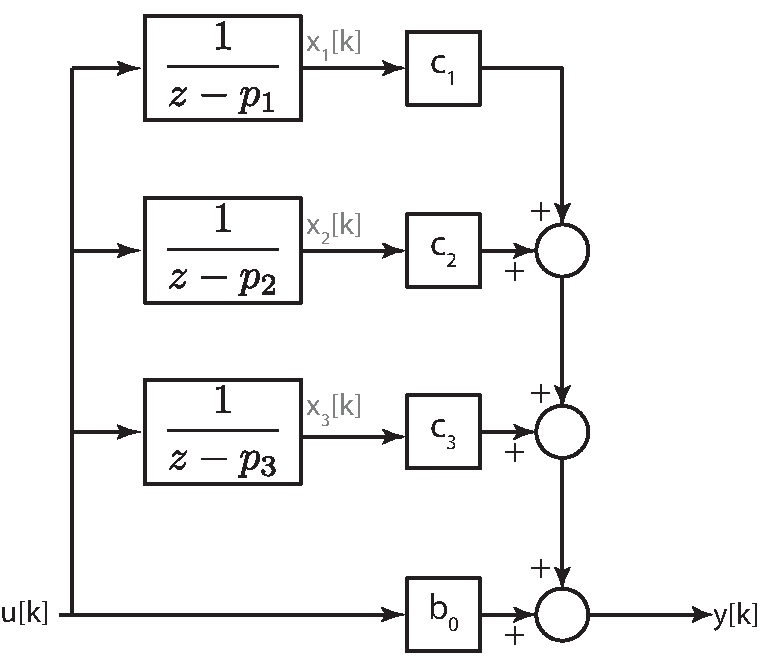
\includegraphics[width=\textwidth]{diagonal}
     \end{center}
 \end{minipage}
     \end{center}
%
Now let's concentrate on the candidate ``state variables''
and try to write state evaluation equations
%
\begin{align*}
X_1(z) &= \frac{1}{z - p_1} U(z) \quad \rightarrow \quad x_1[k+1] = p_1
  x_1[k] + u[k]
\\
X_2(z) &= \frac{1}{z - p_2} U(z) \quad \rightarrow \quad x_2[k+1] = p_2
  x_2[k] + u[k]
\\
X_3(z) &= \frac{1}{z - p_3} U(z) \quad \rightarrow \quad x_3[k+1] = p_3
  x_3[k] + u[k]
\end{align*}
%
where as output equation can be derived as
%
\begin{align*}
y[k] &= b_0 u[k] + c_1 x_1[k] + c_2 x_2[k] + c_3 x_3[k]
\end{align*}
%
If we combine the state and output equations, we
can obtain the state space form as
%
%
\begin{align*}
  \mathbf{x}[k+1] &= \left[ \begin{array}{ccc} p_1 & 0 & 0\\ 0 & p_2 & 0
    \\ 0 & 0 & p_3 \end{array} \right] \mathbf{x}[k]
   + 
  \left[ \begin{array}{c} 1 \\ 1
    \\ 1 \end{array} \right] u[k]
\\
y[k] &= \left[ \begin{array}{ccc} c_1 & c_2 & c_3 \end{array} \right]
+ b_0 u[k]
\end{align*}
%
where 
%
\begin{align*}
\mathbf{x} = \left[ \begin{array}{c} x_1[k] \\ x_2[k] \\
x_1[k] \end{array} \right] \quad , \quad
A = \left[ \begin{array}{ccc} p_1 & 0 & 0 \\ 0 & p_2 & 0
    \\ 0 & 0 & p_3 \end{array} \right]
\quad , \quad 
B = \left[ \begin{array}{c} 1 \\ 1
    \\ 1 \end{array} \right]
\quad , \quad
C = \left[ \begin{array}{ccc} c_1 & c_2 & c_3 \end{array} \right]
\quad , \quad
D = b_0
\end{align*}
%

The form obtained with this approach is called
diagonal canonical form. Obviously, this form is
not applicable for systems that has repeated roots.

For a general $n^{th}$ order system with distinct
roots diagonal canonical form has the following 
$A \ ,  B \ ,  C \ , \& \ D$ matrices
%
\begin{align*}
A &= \left[ \begin{array}{ccccc} p_1 & 0 & \cdots & 0 & 0
              \\ 0 & p_2 & \cdots & 0 & 0
\\ \vdots & \vdots & \vdots & \vdots & \vdots
\\ 0 & 0 & \cdots & p_{n-1} & 0
    \\ 0 & 0 & \cdots & 0 & p_n \end{array} \right]
\quad , \quad 
B = \left[ \begin{array}{c} 1 \\ 1 \\ \vdots \\ 1 \\  1
\end{array} \right]
\\ C &= \left[ \begin{array}{ccccc} c_1 & c_2 & \cdots &  c_{n-1} & c_n \end{array} \right]
\quad , \quad
D = b_0
\end{align*}
%

\subsubsection*{Jordan Canonical Form}

Generalization of diagonal canonical
farm is called Jordan canonical form
which handles repeated roots.

In Jordan form the distinct roots has the 
same structure with Diagonal canonical
form. Let's assume that the $3^{rd}$
order pulse transfer function has
three repeated roots. In this case,
we can expand it using partial fraction 
expansion 
%
\begin{align*}
Y(z) &= \frac{b_0 + b_1 z^{-1} + b_2 z^{-2} + b_3 z^{-3}}{1+ a_1
       z^{-1} + a_2 z^{-2} + a_3 z^{-3}} X(z)
\\
&= \left( b_0 + \frac{c_1}{(z - p)^3} + \frac{c_2}{(z - p)^2}
+ \frac{c_3}{z - p} \right) X(z)
\end{align*}
%
It is possible to realize this expanded form in block diagram 
form as given in the Figure below.
%
     \begin{center}
 \begin{minipage}[h]{0.5\linewidth}
     \begin{center}
       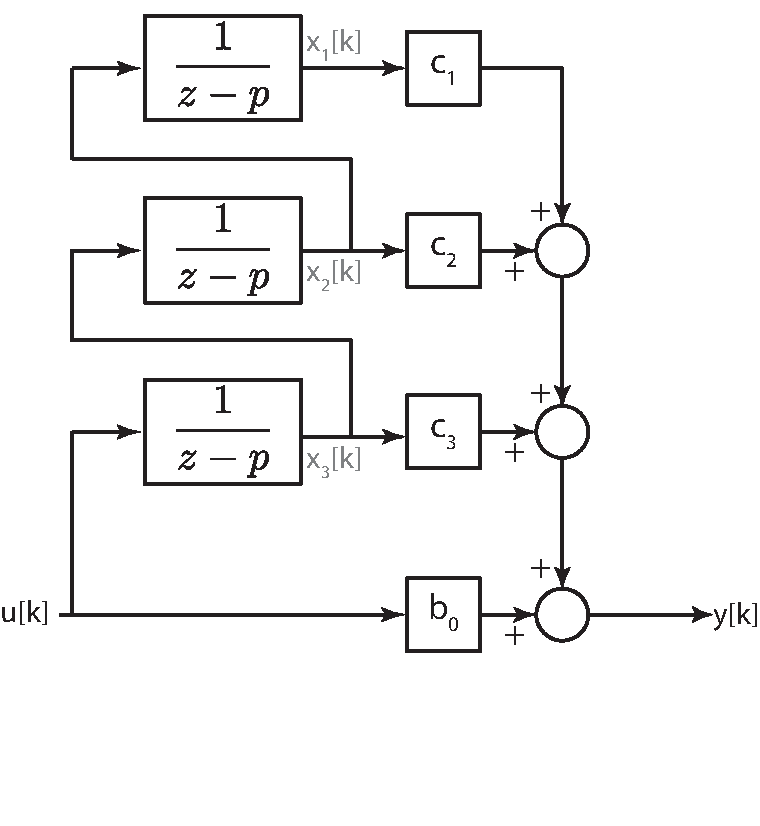
\includegraphics[width=\textwidth]{jordan}
     \end{center}
 \end{minipage}
     \end{center}
%
Now let's concentrate on the candidate ``state variables''
and try to write state evaluation equations
%
\begin{align*}
X_1(z) &= \frac{1}{z - p} X_2(z) \quad \rightarrow \quad x_1[k+1] = p \
  x_1[k] + x_2[k]
\\
X_2(z) &= \frac{1}{z - p} X_3(z) \quad \rightarrow \quad x_2[k+1] = p
         \ x_2[k]
  x_3[k]
\\
X_3(z) &= \frac{1}{z - p} U(z) \quad \rightarrow \quad x_3[k+1] = p \
  x_3[k] + u[k]
\end{align*}
%
where as output equation can be derived as
%
\begin{align*}
y[k] &= b_0 u[k] + c_1 x_1[k] + c_2 x_2[k] + c_3 x_3[k]
\end{align*}
%
If we combine the state and output equations, we
can obtain the state space form as
%
\begin{align*}
  \mathbf{x}[k+1] &= \left[ \begin{array}{ccc} p & 1 & 0\\ 0 & p & 1
    \\ 0 & 0 & p \end{array} \right] \mathbf{x}[k]
   + 
  \left[ \begin{array}{c} 0 \\ 0
    \\ 1 \end{array} \right] u[k]
\\
y[k] &= \left[ \begin{array}{ccc} c_1 & c_2 & c_3 \end{array} \right]
+ b_0 u[k]
\end{align*}
%
where 
%
\begin{align*}
\mathbf{x} = \left[ \begin{array}{c} x_1[k] \\ x_2[k] \\
x_1[k] \end{array} \right] \quad , \quad
A = \left[ \begin{array}{ccc} p & 1 & 0 \\ 0 & p & 1
    \\ 0 & 0 & p \end{array} \right]
\quad , \quad 
B = \left[ \begin{array}{c} 0 \\ 0
    \\ 1 \end{array} \right]
\quad , \quad
C = \left[ \begin{array}{ccc} c_1 & c_2 & c_3 \end{array} \right]
\quad , \quad
D = b_0
\end{align*}
%
$A, \ B, \ \& \ C$ forms a Jordan block. 

For a general $n^{th}$ order system a Jordan block 
with $m$ repeated roots inside a stat-space representation
in Jordan canonical form looks like
%
\begin{align*}
A &= \left[ \begin{array}{c|ccccc|c} 
\ddots & & & & & &
\\ \hline
& \bar{p} & 1 & \cdots & 0 & 0 & 
\\ & 0 & \bar{p} & \cdots & 0 & 0
\\ & & & \ddots & & & 
\\ & 0 & 0 & \cdots & \bar{p} & 1
    \\ & 0 & 0 & \cdots & 0 & \bar{p}
\\
\hline
& & & & & & \ddots
 \end{array} \right]
\quad , \quad 
B = \left[ \begin{array}{c} \vdots \\\hline 
0 \\ 0 \\ \vdots \\ 0 \\  1 \\ \hline
\vdots
\end{array} \right]
\\ C &= \left[ \begin{array}{c|ccccc|c} \cdots & 
c_1 & c_2 & \cdots &  c_{n-1} & c_n & \cdots\end{array} \right]
\end{align*}
%

\subsection*{Similarity Transformations}

Consider the state-space representation of a 
given DT system
%
\begin{align*}
  x[k+1] = G x[k] + H u[k]
\\
  y[k] = C x[k] + D u[k]
\end{align*}
%
Let's define a new ``state-vector'' $\hat{x}$ such that
%
\begin{align*}
  P x[k] = \hat{x}[k] \quad \mathrm{where}
\\
  P \in \mathbb{R}^{n \times n} \quad \mathrm{det}(P) \neq 0
\end{align*}
%
Then we can transform the state-space equations using $P$
as
%
\begin{align*}
  P^{-1} \hat{x}[k+1] = G P^{-1} \hat{x}[k] + H u[k] 
\quad &, \quad y[k] = C P^{-1} \hat{x}[k] + D u[k]
\\
  \hat{x}[k+1] = P G P^{-1} \hat{x}[k] + P H u[k] 
\quad &, \quad y[k] = C P^{-1} \hat{x}[k] + D u[k]
\end{align*}
%
The ``new'' state-space representation is obtained as
%
\begin{align*}
  \hat{x}[k+1] &= \hat{G} \hat{x}[k] + \hat{H} u[k] 
    \\
  y[k] &= \hat{C} x[k] + \hat{D} u[k]
\\
\hat{G} &= P  G P^{-1} \ , \ \hat{H} = P  H \ , \ \hat{C} = C P^{-1} \ ,
  \ \hat{D} = D
\end{align*}
%
Since there exist infinitely many non-singular $n \times n$
matrices, for a given LTI DT system, there exist infinitely 
many different but equivalent state-space representations.

\vspace{24pt}

\textbf{Example:} Show that $A \in \mathbb{R}^{n \times n}$ and $P^{-1} A
P$, where $P \mathbb{R}^{n \times n}$ and $\mathrm{det}(P) \neq 0$, have the
same characteristic equation

\textbf{Solution:} 
\begin{align*}
  \mathrm{det}\left(\lambda I - P^{-1} A P \right) &= 
\mathrm{det}\left( \lambda P^{-1} I P - P^{-1} A P \right)
\\
&= \mathrm{det} \left( P^{-1} \left( \lambda I - A \right) P \right)
\\
&= \mathrm{det} \left( P^{-1} \right)
\mathrm{det} \left( \lambda I - A \right) 
\mathrm{det} \left( P \right)
\\
&= \mathrm{det} \left( P^{-1} \right) \mathrm{det} \left( P \right)
\mathrm{det} \left( \lambda I - A \right) 
\\
\mathrm{det}\left(\lambda I - P^{-1} A P \right) &= \mathrm{det} \left( \lambda I - A \right) 
\end{align*}

\subsection*{Obtaining Transfer Functions from a State-Space
  Representation}

Let's consider the following general state-space form
%
\begin{align*}
  x[k+1] = G x[k] + H u[k]
\\
  y[k] = C x[k] + D u[k]
\end{align*}
%
In order to obtain transfer function form,
we assume that initial conditions are zero.
Under this assumption, let's take z-transform
of both equations
%
\begin{align*}
  z X(z) &= G X(z) + H U(z) 
\quad , \quad
  Y(z) = C X(z) + D U(z)
\\
\left(z I - G \right) X(z) &= H U(z) 
\\
X(z) &= \left(z I - G \right)^{-1} H U(z)
\\
Y(z) &= C \left(z I - G \right)^{-1} H U(z) + D U(z) 
\\
Y(z) &= \left[ C \left(z I - G \right)^{-1} H + D \right] U(z)
\\
T(z) & = \left[ C \left(z I - G \right)^{-1} H + D \right]
\end{align*}
%
If the system is a SISO system, then $T(z)$ is a transfer function,
where as for MIMO case $T(z)$ becomes a \textit{transfer function
  matrix}. Note that $\left(z I - G \right)^{-1}$ is invertible for
all $z \in \mathbb{C}$ except the eigenvalues of $G$. 

\vspace{24pt}

\textbf{Example:} Let $p$ be a pole of $T(z)$, show that
$p$ is also an eigenvalue of $G$. 

\textbf{Solution:} Let 
%
\begin{align*}
  T(z) = \frac{n(z)}{d(z)}
\end{align*}
%
If $p$ is a pole of $T(z)$, then $d(z)|_{p} = 0$. Now let's analyze
the dependence of $T(z)$ to the state-space form. 
%
\begin{align*}
  T(z) &= \left[ C \left(z I - G \right)^{-1} H + D \right]
\\
  \left(z I - G \right)^{-1} &= 
\frac{\mathrm{Adj} \left(z I - G \right) }{\mathrm{det} \left(z I - G
                               \right) }
\\
 T(z) &= \frac{C \mathrm{Adj} \left(z I - G \right) H + D \mathrm{det}
        \left(z I - G
                               \right)}{\mathrm{det} \left(z I - G
                               \right) }
\end{align*}
%
If $p$ is a pole of $T(z)$, then 
%
\begin{align*}
\mathrm{det} \left(z I - G \right)|_{z = p} = 0
\end{align*}
%
Obviously $p$ is an eigenvalue of $G$.

\subsubsection*{Invariance of Transfer Functions Under Similarity
  Transformation}

Consider the two different state-space representations
%
\begin{align*}
  x[k+1] = G x[k] + H u[k]  \quad & \quad \quad \hat{x}[k+1] = \hat{G} \hat{x}[k] + \hat{H} u[k] 
\\
  y[k] = C x[k] + D u[k] \quad & \quad \quad  y[k] = \hat{C} x[k] + \hat{D} u[k]
\end{align*}
%
where they are related with the following similarity transformation
%
\begin{align*}
P x[k] = \hat{x}[k] \ , \
\hat{G} &= P  G P^{-1} \ , \ \hat{H} = P  H \ , \ \hat{C} = C P^{-1} \ ,
  \ \hat{D} = D
\end{align*}
%
Let's compute the transfer function for the second representation
%
\begin{align*}
  \hat{T}(z) &= \left[ \hat{C} \left(z I - \hat{G} \right)^{-1} \hat{H}
  + \hat{D} \right]
\\
&= \left[ C P^{-1} \left(z I - P  G P^{-1} \right)^{-1} P H
  + D \right]
\\
&= \left[ C P^{-1} \left( P \left( z I -   G \right) P^{-1} \right)^{-1} P H
  + D \right]
\\
&= \left[ C P^{-1} P \left( z I -   G \right)^{-1} P^{-1} P H
  + D \right]
\\
&= \left[ C \left( z I -   G \right)^{-1} H + D \right]
\\
\hat{T}(z) &= T(z)
\end{align*}

\newpage

\section*{Solution of Discrete-Time State-Space Equations}

Let's first assume that $u[k] = 0$, and find un-driven (homogeneous)
response.
%
\begin{align*}
  x[k+1] &= G x[k] \\
  y[k] &= C x[k]
\end{align*}
%
Unlike CT systems we can compute the response iteratively
%
\begin{align*}
  x[1] &= G x[0] 
  \\
  x[2] &= G x[1] = G^2 x[0] 
  \\
  x[3] &= G x[2] = G^3 x[0] 
  \\
  \vdots
  \\
  x[k] &= G x[k-1] = G^k x[0] \quad , \quad y[k] = C G^k x[0]
\end{align*}
%
It is easy to see that for $k , p \in \mathbb{Z}$ where $k > p$
%
\begin{align*}
  x[k] &= G^{k-p} x[p] 
\end{align*}
%
Let $\Psi(k) = G^k$, then this matrix of functions solves the
homogeneous difference equation
%
\begin{align*}
  x[k+1] &= G x[k] 
\\    
\\
  x[k] &=\Psi[k] x[0] 
\\
  x[k] &=\Psi[k-p] x[p] 
\\
 x[k+m] &=\Psi[ k + m - m] x[m] = \Psi[k]
\end{align*}
%
$\Psi[k]$ is called the state-transition matrix.
%
Now let's consider input-only state response (i.e. $x[0] = 0$).
%
\begin{align*}
  x[k+1] &= G x[k] + H u[k] 
  \\
  \\
  x[1] &= H u[0]
  \\
  x[2] &= G x[1] + H u[1] = G H u[0] + H u[1] 
  \\
  x[3] &= G x[2] + H u[2] = G^2 H u[0] + G H u[1] + H u[2]
  \\
  x[4] &= G x[3] + H u[3] = G^3 H u[0] + G^2 H u[1] + G H u[2] + H
         u[3]
  \\
  \vdots
 \\
  x[k] &= G x[k-1] + H u[k-1] \\
         &= G^{k-1} H u[0] + G^{k-2} H u[1] +
         \cdots + G H u[k-2] + H u[k-1]
         \\
         &= \left[ \begin{array}{c|c|c|c|c} G^{k-1} H & G^{k-2} H &
         \cdots & G H & H \end{array} \right]
         \left[ \begin{array}{c}
                  u[0] \\ u[1] \\ \vdots \\ u[k-2] \\ u[k-1]
         \end{array} \right]
         \\
         &= \sum\limits_{j = 0}^{k-1} G^{k-j-1} H u[j]
         \\
         &= \sum\limits_{j = 0}^{k-1} G^{j} H u[k-j-1]
\end{align*}
%
Given that $\Psi[k] = G^k$
%
\begin{align*}
    x[k] &= \sum\limits_{j = 0}^{k-1} \Psi[k-j-1] H u[j]
\\
&= \sum\limits_{j = 0}^{k-1} \Psi[j] H u[k-j-1]
\end{align*}
%
If we combine homegeneous and driven responses we can simply obtain
%
\begin{align*}
    x[k] &= \Psi[k] x[0] + \sum\limits_{j = 0}^{k-1} \Psi[k-j-1] H u[j]
\\
&= \Psi[k] x[0] + \sum\limits_{j = 0}^{k-1} \Psi[j] H u[k-j-1]
\end{align*}
% 
whereas output at time $k$ has the form
%
\begin{align*}
    y[k] &= C \Psi[k] x[0] + C \left( \sum\limits_{j = 0}^{k-1}
           \Psi[k-j-1] H u[j] \right) + D u[k]
\\
&= C \Psi[k] x[0] + C \left( \sum\limits_{j = 0}^{k-1} \Psi[j] H
  u[k-j-1] \right) +  D u[k]
\end{align*}
% 

\subsection*{Z-domain Solution of State-Space Equations}

We already computed the transfer function under zero initial
conditions.
%
\begin{align*}
  Y(z) =  \left[ C \left(z I - G \right)^{-1} H + D \right] U(z)
\end{align*}
%
Now let's compute the response to initial condition in Z-domain.
%
\begin{align*}
\mathcal{Z} \left[ x[k+1] \right] &= \mathcal{Z} \left[ G x[k] \right]
\\
z X(z) - z x[0] &= G X(z)
\\
\left( z I - G \right) X(z) &= z X(z) 
\\
X(z) &= z \left( z I - G \right)^{-1} x[0]
\end{align*}
%
Similarly $Y(z)$ takes the form
%
\begin{align*}
  Y(z) &= z C \left( z I - G \right)^{-1} x[0]
\end{align*}
%
We can also observe that
%
\begin{align*}
  \mathcal{Z} \left[ \Psi[k] \right] &= \mathcal{Z} [ G^k ] =
  z \left( z I - G \right)^{-1}
\\
  \mathcal{Z}^{-1} [   z \left( z I - G \right)^{-1} ] &= \Psi[k] = G^k
\end{align*}
%
If we expand $z \left( z I - G \right)^{-1}$ by long ``division'' we
can also observe the relation in z-domain and time doman expressions
from a different perspective
%
     \begin{center}
 \begin{minipage}[h]{0.5\linewidth}
     \begin{center}
       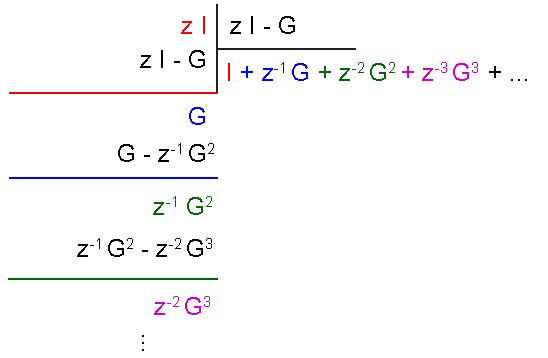
\includegraphics[width=\textwidth]{directdivision}
     \end{center}
 \end{minipage}
     \end{center}
%
\begin{align*}
z \left( z I - G \right)^{-1} &= I + z^{-1} G + z^{-2} G^2 + z^{-3} G^3
  + \cdots
\\
\mathcal{Z}^{-1} \left[ z \left( z I - G \right)^{-1} \right] &=
I \, \delta[k] + G \, \delta[k-1] + G^2 \, \delta[k-2] + G^3 \,
  \delta[k-3] + \cdots 
\end{align*}
%

\newpage

\textbf{Example:} Consider the following state-space representation
%
\begin{align*}
  x[k+1] &= \left[ \begin{array}{ccc} 1 & 0 & 0\\ 0 & 1/2 & 0
    \\ 0 & 0 & -1 \end{array} \right] x[k] 
    + \left[ \begin{array}{c} 1 \\ 1 \\ 1\end{array} \right] u[k]
\\
 y[k] &= \left[ \begin{array}{ccc} 1 & 2 & 3 \end{array} \right] x[k] 
\end{align*}
%
\begin{itemize}
  \item Compute the closed form expression $\Psi[k]$ using the time
   expression

    \textbf{Solution:} The state-space representation is in Diagonal
    canonical form
    
\begin{align*}
  \Psi[k]  = G^k = \left[ \begin{array}{ccc} 1 & 0 & 0\\ 0 & 1/2 & 0
    \\ 0 & 0 & -1 \end{array} \right]^k 
    = \left[ \begin{array}{ccc} 1^k & 0 & 0\\ 0 & (1/2)^k & 0
    \\ 0 & 0 & (-1)^k \end{array} \right]
 = \left[ \begin{array}{ccc} 1 & 0 & 0\\ 0 & (1/2)^k & 0
    \\ 0 & 0 & (-1)^k \end{array} \right]
\end{align*}    

\item Compute the closed form expression $\Psi[k]$ using the z-domain 
  solution method

\textbf{Solution:}

\begin{align*}
  \Psi[k]  &= \mathcal{Z}^{-1} \left[   z \left( z I - G \right)^{-1} \right]
\\
&= \mathcal{Z}^{-1} \left[   z \left( \left[ \begin{array}{ccc} z-1 & 0 & 0\\ 0 & (z-1/2) & 0
    \\ 0 & 0 & z+1 \end{array} \right] \right)^{-1} \right]
\\
&= \mathcal{Z}^{-1} \left[   \left[ \begin{array}{ccc} \frac{z}{z-1} & 0 & 0\\ 0 & \frac{z}{z-1/2} & 0
    \\ 0 & 0 & \frac{z}{z+1} \end{array} \right] \right]
\\
&= \left[ \begin{array}{ccc} 1 & 0 & 0\\ 0 & (1/2)^k & 0
    \\ 0 & 0 & (-1)^k \end{array} \right] \quad \mathrm{for} k \geq 0
\end{align*}    

\item Compute the impulse response of the system from the time domain
solution

\textbf{Solution:}

\begin{align*}
  x[k] &= G^{k-1} H u[0] \quad \mathrm{for} \  k > 0 \\
  y[k] &= C G^{k-1} H \quad \mathrm{for} \ k > 0 \\ 
         &= \left[ \begin{array}{ccc} 1 & 2 & 3 \end{array} \right] 
                \left[ \begin{array}{ccc} 1 & 0 & 0\\ 0 & (1/2)^{k-1} & 0
    \\ 0 & 0 & (-1)^{k-1} \end{array} \right]
      \left[ \begin{array}{c} 1 \\ 1 \\ 1\end{array} \right] 
\\
&= \left[ \begin{array}{ccc} 1 & 2 & 3 \end{array} \right] 
\left[ \begin{array}{c} 1 \\ (1/2)^{k-1} \\ (-1)^{k-1} \end{array}
  \right] 
\\
y[k] &= 1 + 2 (1/2)^{k-1} + 3 (-1)^{k-1} \quad \mathrm{for} \ k > 0 
\end{align*}    

\item Compute the transfer function $\frac{Y(z)}{U(z)}$

\textbf{Solution:}

\begin{align*}
  T(z) &= C \left( z I - G \right)^{-1} H \\
         &= \left[ \begin{array}{ccc} 1 & 2 & 3 \end{array} \right] 
\left[ \begin{array}{ccc} z-1 & 0 & 0\\ 0 & z-1/2 & 0
    \\ 0 & 0 & z+1 \end{array} \right]^{-1}           
\left[ \begin{array}{c} 1 \\ 1 \\ 1\end{array} \right]
\\
&= \left[ \begin{array}{ccc} 1 & 2 & 3 \end{array} \right] 
\left[ \begin{array}{ccc} \frac{1}{z-1} & 0 & 0\\ 0 & \frac{1}{z-1/2} & 0
    \\ 0 & 0 & \frac{1}{z+1} \end{array} \right]           
\left[ \begin{array}{c} 1 \\ 1 \\ 1\end{array} \right]                                   
\\
&= 
\left[ \begin{array}{ccc} 1 & 2 & 3 \end{array} \right] 
\left[ \begin{array}{c} \frac{1}{z-1} \\ \frac{1}{z-1/2} \\
         \frac{1}{z+1}\end{array} \right]         
\\
  T(z) &= \frac{1}{z-1} + \frac{2}{z-1/2} + \frac{3}{z+1}
\end{align*}    

\item Compute the inverse Z-transform of the  transfer function 

\textbf{Solution:}

\begin{align*}
  t[k] &= \mathcal{Z}^{-1} \left[ \frac{1}{z-1} + \frac{2}{z-1/2} +
  \frac{3}{z+1} \right]
\\
&= \left( 1 + 2 (1/2)^{k-1} + 3 (-1)^{k-1} \right) h[k-1]
\end{align*}    
%
where $h[k]$ is the unit step function


\end{itemize}

% **** This ENDS THE EXAMPLES. DON'T DELETE THE FOLLOWING LINE:
\end{document}